\chapter{Environment Modeling and Abstraction of Network States}
	\label{cha:ema}
	
   	\acp{CAN} promise to overcome the shortcomings of \ac{SON} implementations, i.e., the limited flexibility and adaptability to changing environments, by applying cognition.
   	In \ac{CAN}, intelligent network automation functions -- called \acp{CF} -- apply machine learning techniques to learn context-specific behavioral policies with which to automate network operations.
   	For proper operation, the \ac{CAN} system needs to learn the environment in which the functions are operating and to abstract the environment and performance observations into network states, which the \acp{CF} can use to communicate and respond to.
   	
   	As discussed previously, quantization algorithms are primarily designed for this exact purpose: the automatic partitioning of a state-space into a finite number of discrete states, and the selection of a representative observation for each state.
   	These states can then be used as a vocabulary for cognitive functions in the mobile network, upon which decisions or requests can be based.
   	However, the problem in this scenario is a bit more complicated, since the \ac{CAN} concept presumes a large amount of varied information communicated this way, in order to facilitate the consideration of a larger context in the decision making.
   	On one hand, this poses a challenge to the quantization algorithms, which would need to work in an extremely high-dimensional space if applied as-is on the network data.
   	Unfortunately, even though the previously described quantization algorithms try to avoid the curse of dimensionality by forming quanta that is independent of the number of dimensions, they all would eventually run into problems stemming from dimensionality.
   	On the other hand, it is quite likely that some of the information is redundant and could be abstracted away into a more dense, simplified description.
   	Thus, the goal here is to both encode the original network state-space into an abstracted state-space, and define discrete (abstract) network states within it.
   	This chapter discusses the design, implementation and evaluation of an \ac{EMA} engine that could be tasked to define these abstract network states in a consistent way across multiple \acp{CF}.
   	
	Sec.~\ref{cha:ema:sec:ema} introduces the \ac{EMA} concept in detail by taking elements from the following patent application:
   	
	\begin{patent}
		Environment Modeling and Abstraction of Network States for Cognitive Functions \\
		\textit{Benedek Schultz, Márton Kajó, Stephen S. Mwanje} \\
		WO, PCT application no.: PCT/EP2018/069638, filed July 2018
	\end{patent}

	Sec.~\ref{cha:ema:sec:ema_bsq} discusses the implementation and evaluation of an \ac{EMA} module by detailing the work published in the following paper:

	\begin{publication}
		Environment modeling and abstraction of network states for cognitive functions \\
		\textit{Stephen S. Mwanje, Márton Kajó, Sayantini Majumdar, Georg Carle} \\
		NOMS 2020-2020 IEEE/IFIP Network Operations and Management Symposium, pp. 1-8. IEEE, 2020.
	\end{publication}	

	My contributions to the above paper was the design of the \ac{EMA} module and its relevant algorithms, the design of the evaluation, the supervision of the implementation and the evaluation, as well as the co-authoring of the paper.
	The discussion in this thesis expands on the paper by connecting it to my previous works (Cha.~\ref{cha:quantization}), which give more detail for the specific clustering algorithms used, as well as connecting it to subsequent research published in the following paper:

	\begin{publication}
		Modeling and Abstraction of Network and Environment States Using Deep Learning \\
		\textit{Stephen S. Mwanje, Márton Kajó, Janne Ali-Tolppa} \\
		IEEE Network 34, no. 6 (2020): 8-13.
	\end{publication}	
	
   	Sec.~\ref{cha:ema:sec:ema_acai} details the work published in the above paper, where my contribution was the reimplementation of all evaluated algorithms, the evaluation and the co-authoring of the paper.   	

	\section{Concept: EMA in Cognitive Autonomous Networks}
		\label{cha:ema:sec:ema}
	
		\subsection{Elements of Cognitive Autonomous Networks}
			
			The concept of applying cognition to \ac{NM} has been advanced in several publications, including \cite{can_q_learning, can_challenges}, which propose to replace the hard-coded logic in \ac{SON} functions with highly intelligent, adaptive \acp{CF}. 
			The \acp{CF} should be capable of learning optimal behavior based on their actions and the observed impact on the network, network environment and other \acp{CF}, by processing various data, such as configuration, performance, failure, or user/service-related indicators.			
			If these \acp{CF} are in place, the evolved system would result in what has been labeled in our nomenclature as a \ac{CAN}.
			In effect, \ac{CAN} extends \ac{SON} to: 1) be able to infer higher level network and environment states from a multitude of data sources instead of the current low-level basic states recovered from \acp{KPI} values, and 2) allow for adaptive selection and changes of network configuration parameters depending on previous actions and operator goals.
			
			\begin{figure}[ht]
				\centering
				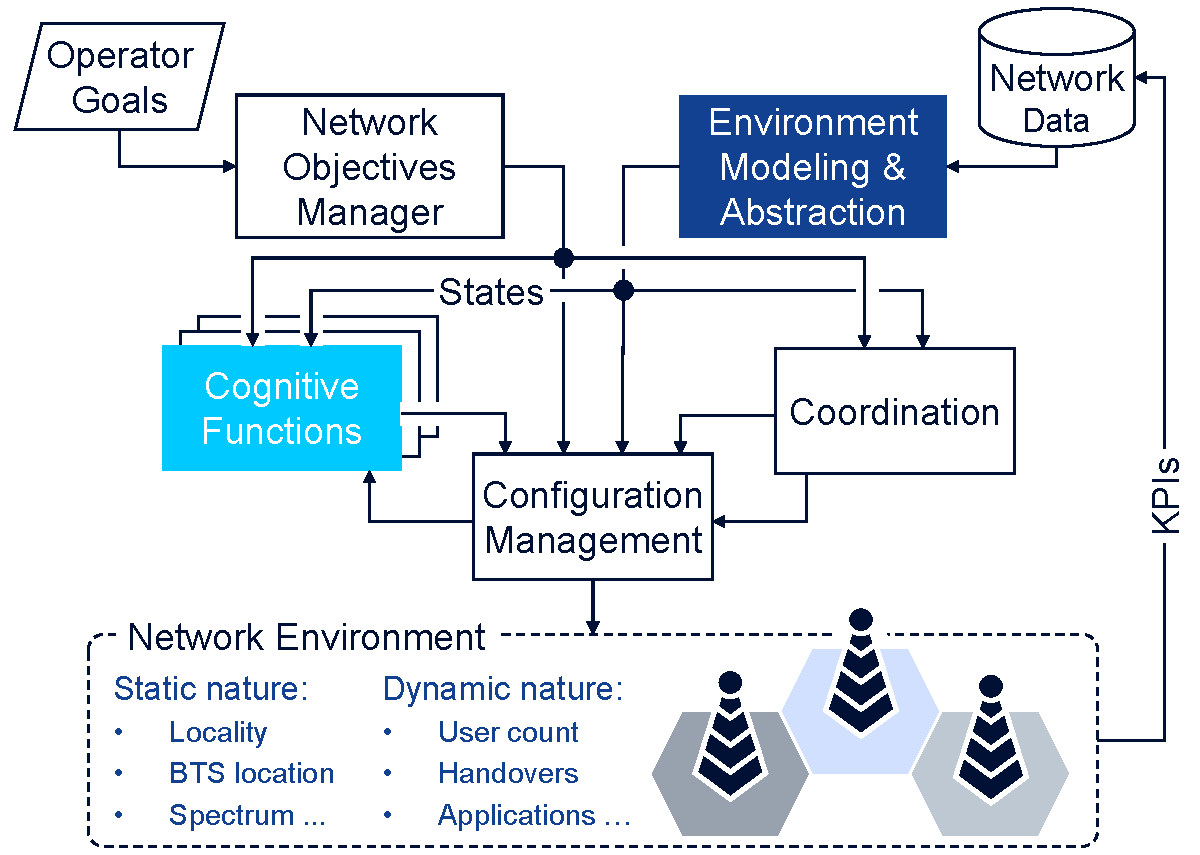
\includegraphics[width=0.8\linewidth]{figures/04_ema/can_overview/can_overview.pdf}
				\caption[CAN components]{The components of a Cognitive Autonomous Network.}
				\label{fig:can_overview}
			\end{figure}
		
			The \ac{CAN} framework proposed in \cite{can_itu} highlights where and how cognition should be introduced into the \ac{NM} system.
			The framework, shown in Fig.~\ref{fig:can_overview}, proposes five major components.
			A \ac{NOM} translates the operator objectives into a set of more concrete \ac{KPI} targets for the other CAN subsystems. 
			Each \ac{CF} then tries to optimize the network configuration to achieve the defined \ac{KPI} targets or its own subset thereof. 
			Since there are typically many independent \ac{CF} instances acting in a \ac{CAN}, a component called the \ac{CE} is required to coordinate their actions and to prevent any possible conflicts. 
			To achieve this, the \ac{CE} may need to know the dependencies between the \ac{CF} instances and their actions, which may be partially learned.
			The actions selected to be implemented are then deployed by the \ac{CME}, which may be combined with the \ac{CE}.
			The \ac{CME} takes care of scheduling the deployment of the actions and verifying that they are successfully taken.
			Each \ac{CF} responds to specific states in the network that may be different among the \acp{CF}, e.g. a handover optimization CF responds to mobility profiles in the cells, while a congestion management \ac{CF} may consider the load in different cells and/or network slices. 
			Moreover, the states may need to be communicated among entities, e.g. between the \acp{CF} and the control or coordination modules.
			So, an \ac{EMA} engine is required to model and abstract the network environment into discrete states, which are consistent across the components.
			This way the components are able to communicate to each other with reference to the same state space.
			
		 \subsection{Environment Modeling and Abstraction Engine}
		 
	 		A common understanding of the network states is critical to efficient operation of cognitive functions.
	 		To illustrate this, consider two \acp{CF}, CF$_A$ and CF$_B$, e.g. interference management and coverage optimization. 
		 	These cognitive functions need to exchange information about their observations to improve their learning, as they are affecting shared network parameters, and have overlapping goals.
		 	CF$_A$ takes an action at three time points $t_1$, $t_2$ and $t_3$ for which CF$_B$ notices different effects: $t_1$ and $t_3$ are unacceptable, $t_2$ is good.
		 	CF$_B$ wishes to inform CF$_A$ about its perception of the actions. 
		 	Without a common understanding of the network states, CF$_B$ must enumerate all its observations as tuples of times and measurements, which might or might not be understandable by CF$_A$.
		 	However, knowing that at $t_1$ and $t_3$, the network state was the same and knowing the label simplifies the exchange.
		 	This way, CF$_B$ can simply encode that “in state $S_1$, action $a$ always leads to unacceptable outcomes”, simplifying communication and removing complexity from both \acp{CF}.
		 	
	 		% Observable Network State	ONS
		 	% EMA-Internal State		EIS
		 	% Discrete Abstract State	DAS
		 	
	 		The network and its environment presents an \ac{ONS}, which is encoded into an $n$-dimensional vector of data on observed environmental conditions, configurations and the subsequently measured \acp{KPI}.
		 	The \ac{EMA} engine must take such observable network state vectors and abstract them into outputs called \ac{DAS}, to which the \acp{CF} respond.
 			Specifically, the \ac{EMA} defines abstract states built from combinations of quantitative \acp{KPI}, abstract (semantic) state labels and operational contexts, such as the current configurations of the network or its elements.
		 	These states are discretized to simplify the communication between the various modules in the \ac{CAN}. 
		 	The abstract labeling of network states must be done in a consistent way across multiple \acp{CF} in a \ac{CAN}, to ensure that the modules reference the same abstract states when communicating to each other, e.g., for the Coordination Engine to inform the \acp{CF} about the effects of their actions to one another. 
		 	As such, the \ac{EMA} generates a Discrete Abstract state vector $S$ of dimension $m$, representing the (quasi-orthogonal) features of interest for the active \acp{CF}, e.g., the optimization of cell load, energy consumption, etc.
		 	
		 	The proposed implementation of the \ac{EMA} can be seen in Fig.~\ref{fig:ema_overview}.
		 	The \ac{EMA} has $2$ modules: the \ac{EMM}, and the \ac{SAM}.	
		 	The goal of the \ac{EMM} is to split the $n$-dimensional continuous input space into $k$ discrete volumes (quanta), which can be assigned with different labels in the \ac{SAM}. 
		 	To realize this, during training, the \ac{EMM} creates an \ac{EISS} of $k$ \acp{EIS} as the complete, but simplified view of the network environment.		 	
		 	Objectivity means that the \ac{EISS} can not incorporate possibly biased information during training, such as expert knowledge from the operator or requirements from \acp{CF}, i.e; the \ac{EISS} has to be formed purely on \acp{ONS}, in an unsupervised manner.		 	
		 	Objectivity is needed in order to minimize the need for relearning the \ac{EISS} in case of changes in the active \acp{CF} or the requirements thereof.		 	
		 	Moreover, the \ac{EISS} must have a good resolution to ensure support for different levels of granularity at abstraction. 
		 	These requirements make environment modeling a quantization task.
		 	Since it can be expected that some of the input dimensions contain noise or redundant information, it is beneficial to precede the quantization step with a feature extractor, which removes these interfering parts of the data.
		 	Because both feature extraction and quantization only aims to model structure that is already present in the data (no additional expert knowledge or context need to be added), both functions are trained through unsupervised means.
		 	The quantized nature of the state-space makes it easy to append this contextual information later, which is the task of the \ac{SAM}.
		 	
		 	\begin{figure}[ht]
		 		\centering
		 		\subfloat[Concept]{
		 			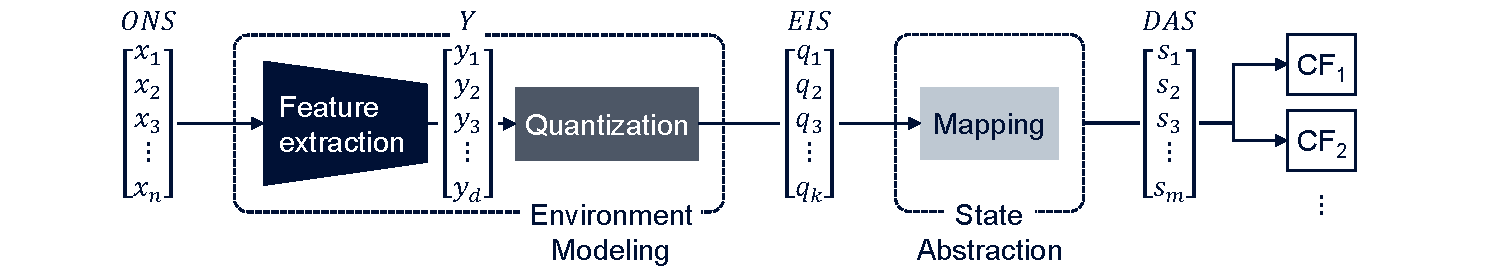
\includegraphics[width=\linewidth]{figures/04_ema/ema_overview/ema_overview_concept.pdf}
		 		} \\
		 		\subfloat[Implementation]{
		 			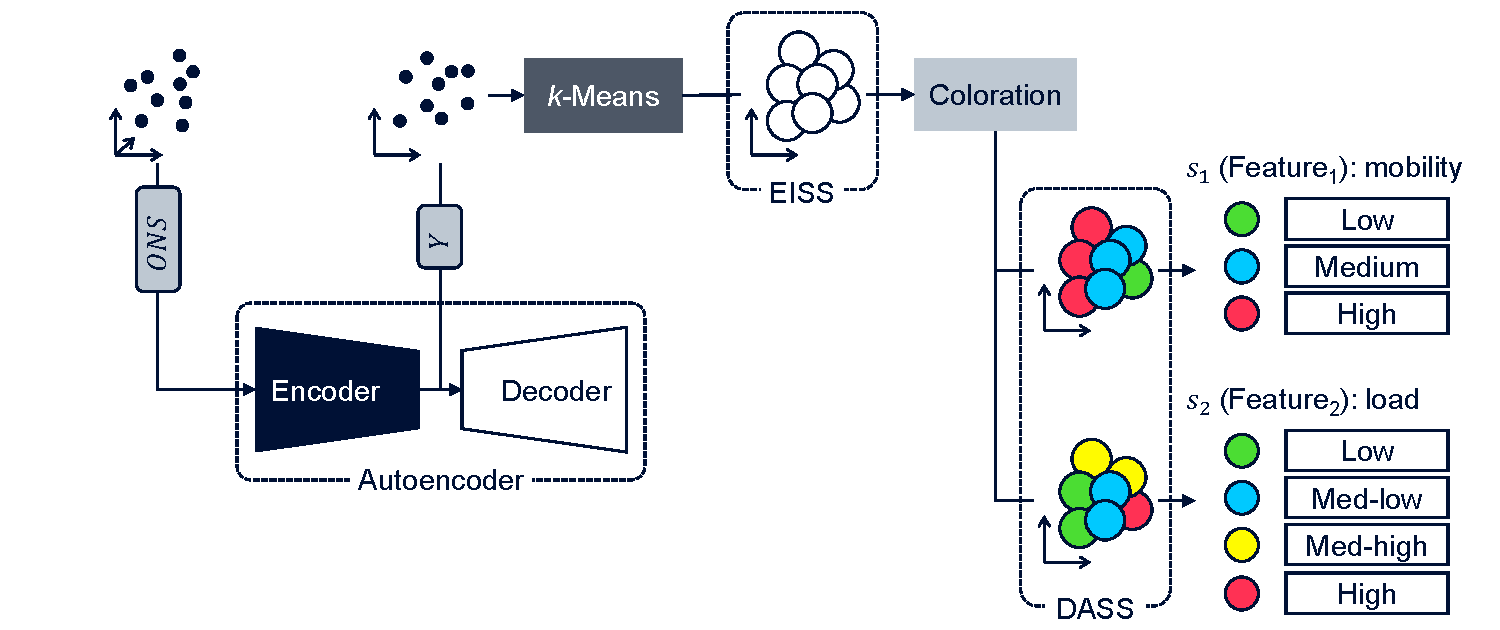
\includegraphics[width=\linewidth]{figures/04_ema/ema_overview/ema_overview_implementation.pdf}
		 		}	 		
		 		\caption[EMA components]{The components and input-output vectors of the EMA engine.}
		 		\label{fig:ema_overview}
		 	\end{figure}
		 	
		 	Given the appropriate modeling, the \ac{SAM} appends contextual information to the quanta to create the \ac{DASS} of flexible mappings which can be modified during run-time.
		 	This bridges the gap between the objective \ac{EISS} and the subjective \ac{DASS}, whose states are specific to the active \acp{CF}.
		 	For each output feature, possibly corresponding to a specific \ac{CF}, the state abstraction stores a labeling (coloration) of the size-$k$ internal states resulting in at most $k$ individual values for each of the $m$ output dimensions.
		 	The coloration contains expert knowledge or context information required for the \acp{CF}, implying that state mapping: 1) is trained in a supervised or semi-supervised manner, owing to the need for feedback about the utility of the learned labels for the \acp{CF}; and 2) is reconfigurable since the \acp{CF}' requirements or settings are likely to change.
		 	
			It is critical to align the quantization to the actual contextual groups (classes) present in the \acp{ONS} (such as measurements from cells with similar parameter settings), in order for the coloration in the \ac{SAM} to be able to map the subjective discrete abstract states to the objective \acp{ONS} with high precision.
		 	If not, the formed quanta may contain a mixture of network states, and labeling such quanta becomes meaningless.
		 	This was the basis of our evaluation of the \ac{EMA} concept, which is detailed in the following.	
		 	
		 \subsection{Related Work}
		 
 			The modeling of a system's states is of great interest in studies on complex systems.
 			System-state modeling has been studied in generic autonomous systems, such as in \cite{model_hazard_phd}, and in cyber-security systems, e.g., to characterize the behavior of attack systems, such as in \cite{model_relab_optim, model_defense}.
 			The most widely studied systems-states are in robotic control systems where a controller may wish to identify the different states of the underlying system and how to respond to such states \cite{model_sonar_robot, model_wheeled_robot}.
 			The typical challenge here is to derive a closed form description of the different features of the robotic system, e.g. to characterize the angular position, angular velocity and armature current in the case of motion control of an electric motor \cite{model_fpga_pid}.
		 	
		 	There has, however, been little work on modeling states in communication networks.
		 	Typically, theoretical system models are developed to study the behavior of the wireless network in particular conditions, the most widely documented models being in wireless sensor networks \cite{model_routing, model_lmac}.
		 	However, these do not model the different states in which the system may be or their interaction with the environment or control conditions.
		 	This is also the case for communication network management automation.
		 	
		 	The concept of network states and their inference in self-organizing networks for enabling \ac{5G} have been treated in \cite{qi_anomalydet}.
		 	Similar to our work, the authors propose a framework responsible for selecting a set of metrics to characterize the network states, reducing the dimensionality of the data using \ac{PCA} and applying a semi-supervised classification algorithm, suited to deal with unambiguous knowledge about the classes.
		 	Although this paper adopts a similar algorithmic framework in the sequence of dimension reduction and clustering using semi-supervised Fuzzy C-Means, it is solely applied to the anomaly detection use case.
		 	
		 	The authors in \cite{borislava_improved} also propose an improved anomaly detection framework by dynamically learning mobile network cell states using the \ac{MGNG} algorithm.
		 	The baseline is set to be the \acp{KPI} of individual cells fed to the \ac{MGNG} algorithm, in order to determine shared or common behavior of the cells, an approach which the data processing steps in our study follow.

	\section{EMA using Bounding Sphere Quantization}
		\label{cha:ema:sec:ema_bsq}
	
		\subsection{Simulation Environment and Data}
		
			In order to numerically evaluate the proposed \ac{EMA} concept, a dataset from a controlled network and environment is needed, one that contains known classes (groups) that are discoverable by the environment modeling system.
			To generate such a dataset, a realistic system-level simulator was used, in order to be able to model a complex network scenario.
			The classes for the evaluation were formed by cells sharing similar parameter setting combinations. 
			Although this is not entirely realistic, as cell parameter settings would be known to the operator in a real network deployment, it helps us evaluate the EMA concept; the parameters are meant to mimic different user behaviors and environmental conditions that might affect the network and are outside of the operators control.
			
			To model a realistic heterogeneous network, the simulation scenario contained a number of $3$-sector \ac{LTE} macro ($2$ GHz), omnidiricetional \ac{LTE} micro ($2.6$ GHz), and WiFi ($2.4$ GHz) cells.
			Three parameters were iterated to form $12$ setting groups (classes) as shown in Tab.~\ref{tab:cell_params_1}, these were the \ac{RSRP} offset, \ac{TTT} and \ac{TXP}.
			The simulator used the WINNER+ propagation model \cite{winner_plus} for coverage, interference and fading calculations.
			It evaluates vehicular and pedestrian users both moving along randomized routes on prerecorded paths in a digital recreation of the city of Helsinki, all the while simulating different activities, such as \ac{FTP} downloads, video and \ac{VoIP} calls.
			
			\begin{table}[t]
				\renewcommand*{\arraystretch}{1.2}
				\centering
				\begin{tabular} {l|c c c c c c c c}
										& \multicolumn{8}{c}{LTE Macro} \\ 
					\hline
					Setting 			& M$_{1}$	& M$_{2}$	& M$_{3}$	&	M$_{4}$	& M$_{5}$	& M$_{6}$	& M$_{7}$	& M$_{8}$	\\
					\hline 
					RSRP offset [dB] 	& 2.0		& 3.0		& 3.0		& 2.0		& 2.0		& 3.0		& 3.0		& 2.0		\\
					TTT [s]				& 0.512		& 0.512		& 0.512		& 0.512		& 0.64		& 0.64		& 0.64		& 0.64		\\
					TXP [dBm]			& 46		& 46		& 40		& 40		& 46		& 46		& 40		& 40		\\
					\hline						
										& \multicolumn{2}{c|}{LTE micro} 			& \multicolumn{2}{c}{WiFi} 			& & & & \\
					\cline{1-5}
					Setting 			& m$_1$	& \multicolumn{1}{c|}{m$_2$}		& W$_1$	& \multicolumn{1}{c}{W$_2$}	& & & & \\
					\cline{1-5} 
					RSRP offset [dB] 	& 2.0	& \multicolumn{1}{c|}{2.0}			& -		& \multicolumn{1}{c}{-}		& & & & \\
					TTT [s]				& 0.512	& \multicolumn{1}{c|}{0.64}			& 0.512	& \multicolumn{1}{c}{0.64}	& & & & \\
					TXP [dBm]			& 20	& \multicolumn{1}{c|}{20}			& 20	& \multicolumn{1}{c}{20}	& & & & \\
				\end{tabular}
				\caption[Cell parameters in the EMA simulation]{Cell parameter combinations in the simulation.}
				\label{tab:cell_params_1}
			\end{table}

			The output of the simulator is made up of measurements at the cell transceiver level.
			Generally, three categories of output measurements were observed, an overview of which can be found in Tab.~\ref{tab:kpi_types} with examples.
			These measurements were used in subsequent data preprocessing steps to bring the raw simulation data into a form intelligible to machine learning algorithms (specifically neural nets).
			The data pertaining to a single cell was enriched by appending the aggregated properties (\acp{KPI}) of its neighbors, essentially considering \textit{shared} characteristics of the cells in the network.
			The simulator worked with a simulation step of $0.1$ ms, outputting these measurements too frequently for network management use.
			To rectify this, all measurements were aggregated in time to $15$ second intervals.
			Finally, the resulting dataset was normalized per feature across all timestamps and cells.
			The end result of the preprocessing is a clean, standardized dataset consisting of two kinds of information: identifiers in integer form, and \acp{KPI} in floating point values.
			The dataset, which serves as input to the \ac{EMA}, did not include network configuration details in any quantity (which would directly correspond to the classes).
			With all this, the final dataset contained $34$ features altogether.
			
			\begin{table}[t]
				\renewcommand*{\arraystretch}{1.2}
				\centering
				\begin{tabular}{p{0.2\linewidth}|p{0.3\linewidth}|p{0.4\linewidth}}
					Type				& Description									& Example \\ 
					\hline
					\hline
					Cell counters 		& Local events or those in neighbor cells 		& Radio Link Failures (RLFs), Handovers (HOs) \\
					\hline
					Shared counters 	& Events for specific cell pairs 				& RLFs due to late HO from cell $1$ to $2$\\
					\hline
					\acp{KPI}			& \acp{KPI} aggregated to every simulation step & Total number of active \acp{UE}, cell load \\
					\hline
				\end{tabular}
				\caption[KPIs collected from the EMA simulation]{Categories of cell events and measurements (KPIs) collected from the simulation.}				
				\label{tab:kpi_types}
			\end{table}
					
		\subsection{Feature Extraction using an Autoencoder}
			\label{cha:ema:sec:fe}
		
			The \ac{EMA} input is made up of many features (dimensions), each of which embodies an aspect of the network environment.
			In our case, this input was made up of the previously mentioned $34$ features.
			Since it is highly challenging to process or visualize such high-dimensional datasets \cite{curse_of_dim_2}, feature extraction is often used to try to find a better representation to which later machine learning algorithms can be applied effectively.
			Specifically, in our setting, distance-based quantization is susceptible of breaking down in high-dimensional spaces, which warrants the use of feature extraction.
		
			The task of the feature extraction module is to compress the input to a lower-dimensional representation, while also possibly removing redundant information and noise.
			The number of extracted features ($d$) is usually significantly smaller than the number of input features ($d << n$), but using more dimensions ($d >> n$) with sparsity enforced could also be a viable alternative.
			The reduction of features or the enforcement of sparsity usually means a tradeoff between the level of compression and loss of valuable information.
			It is up to the designer to figure out a good tradeoff, which can be specific to the dataset used, or to the later processing steps.
	
			In this work, an \ac{FC} autoencoder neural net (Sec.~\ref{cha:deep_learning:sec:ae}) was used as the feature extractor.
			Autoencoders excel in generalizing underlying logic and structure in the data.
			The more compression is enforced, the more the autoencoder is forced to extract generalization, removing noise and redundancies in the process.
			However, as compression is increased, more and more nuance is lost in the reconstructed data.
			The level of compression is set by the number of neurons in the middle layers (encoding size), as such, different compression levels equate to different topologies.
			Figure~\ref{fig:ae_losses}) shows the reconstruction loss measured on a few autoencoder topologies, with the encoding size highlighted.
			The used autoencoders also utilized a single hidden layer in both the encoder and the decoder, the size of which were set to the average of the number of original and compressed dimensions ($n$ and $d$), so that the progression of compression and decompression in the net is roughly linear.
			In the end, an encoding size of $10$ was chosen, a topology that is a good tradeoff between compression and loss of information for this scenario, equating roughly to a $3x$ compression factor.
			
			\begin{figure}[ht]
				\centering
				\subfloat{
					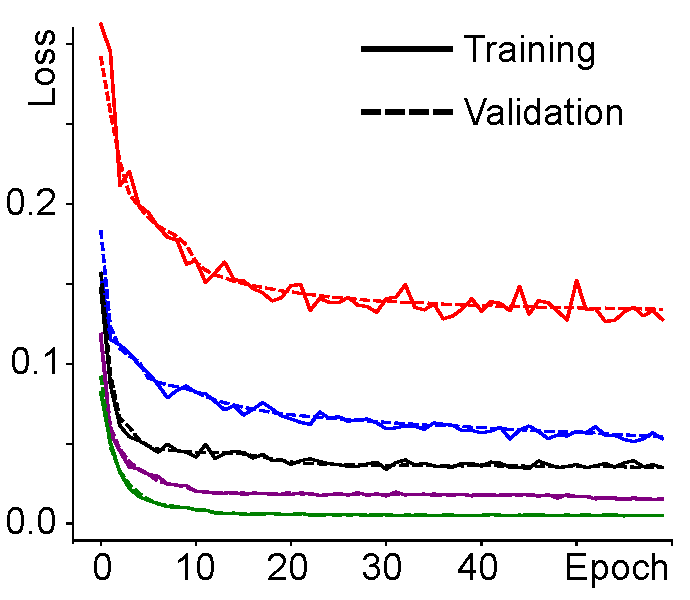
\includegraphics[width=0.38\linewidth]{figures/04_ema/ae_losses/ae_losses_framed.pdf}
				}
				\subfloat{
					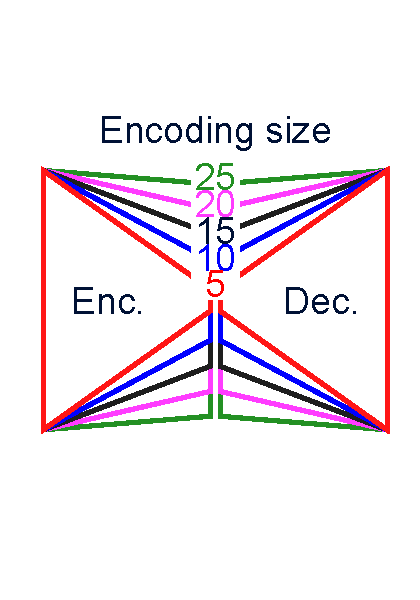
\includegraphics[width=0.22\linewidth]{figures/04_ema/ae_losses/ae_losses_topology.pdf}
				}
				\caption[AE losses for different encoding sizes]{Training and validation loss development during training for different encoding sizes.}
				\label{fig:ae_losses}
			\end{figure}
			
			Figure~\ref{fig:ae_encoding} shows a scatter plot of the encoded observations with the chosen autoencoder topology, using the first $2$ dimensions in the $10$-dimensional encoded space.
			The activations are colored according to the parameter combination of the origin cell.
			Even though the $2$-dimensional scatter plot is incapable of capturing the complexity of the $10$-dimensional space, clustering/grouping of the colors is observable even in this basic visualization.
			As one example -- according to Tab.~\ref{tab:cell_params_1} -- WiFi (and micro) cells could be easily distinguished from the macro cells in terms of transmit power.
			Although transmit power settings were not communicated to the autoencoder, the difference in behavior still makes these cells stand apart from the other measurements.
			This distinction is also captured in the encoding, as the WiFi observations are mostly clustered along the top and left part of the plot, as highlighted by the two respectively colored curves.
		
			\begin{figure}[ht]
				\centering
				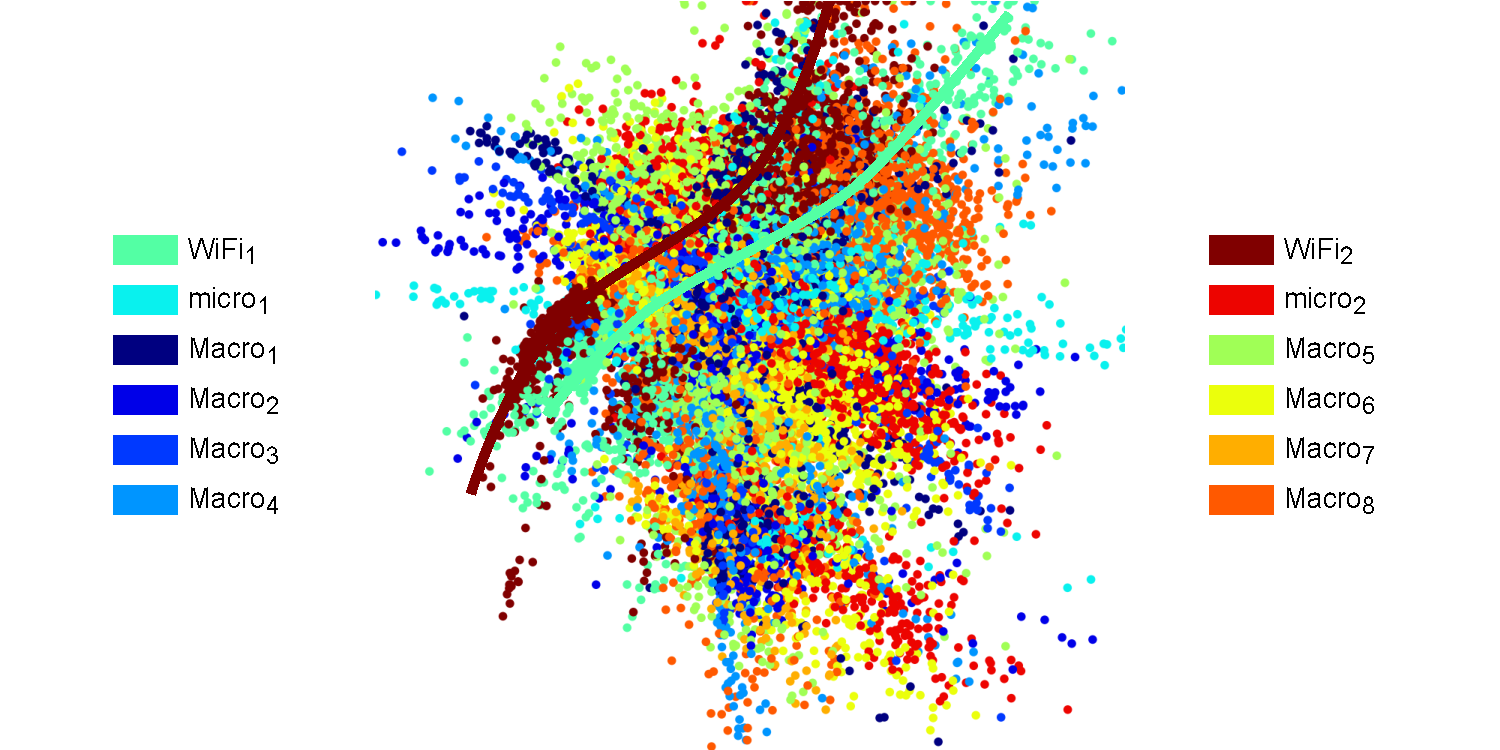
\includegraphics[width=\linewidth]{figures/04_ema/ae_encoding/ae_encoding.pdf}
				\caption[Scatterplot of the encoded measurements in the EMA evaluation]{Scatterplot of encoded measurements taken from cells with the $12$ parameter classes, projected to $2$D using PCA.}
				\label{fig:ae_encoding}
			\end{figure}
		
		\subsection{Quantization with BSQ and $k$-Means}
		
			In this work, two unsupervised clustering algorithms were chosen to be evaluated for the quantization task: our \ac{BSQ} and the traditional Lloyd's \kmeans{} algorithm.
			Instead of using existing packages, both algorithms used the neural-net-style reimplementations as discussed in Sec.~\ref{cha:quantization:sec:nn_quant}.
			These implementations synergize well with the autoencoder, so that the whole processing pipeline of the \ac{EMA} can use the same tools and utilize hardware acceleration.		
			Figure~\ref{fig:ae_fits} depicts the results of running the two algorithms on the autoencoder activations from Sec.~\ref{cha:ema:sec:fe}, by plotting the first $2$ dimensions from the $10$-dimensional space.
			Although these plots lose information that is contained in the remaining eight dimensions when projected to $2$D, they provide a general idea of how the clustering behaves in higher dimensions.
			It is visible that with $k$-Means, quanta are more concentrated around the denser regions of the dataset, while they are more spread out when using \ac{BSQ}.
			
			The two algorithms differ in their end goal when fitting the quantization.
			Quantization being an unsupervised learning problem, it is hard to deduct which algorithm is ``better'' without use case specific supervised metrics.
			This evaluation will be shown in the next section (Sec.~\ref{cha:ema:sec:mapping}).
			However, it is still beneficial to look at unsupervised metrics to get a better understanding how the two algorithms behave.
			We considered two evaluation metrics, which cover the respective global optimization goals of the two algorithms:			
			\begin{itemize}
				\item Average distances are computed by taking the mean of the nonzero masked distances first within each cluster (i.e. along each column), and then for the resulting one-dimensional tensor over all.
				\item Maximum distances are computed by taking the maximum of the nonzero masked distances in each quanta, and afterwards averaging them across quanta.
			\end{itemize}
			
			\begin{figure}[ht]
				\centering
				\subfloat[\kmeans{}]{
					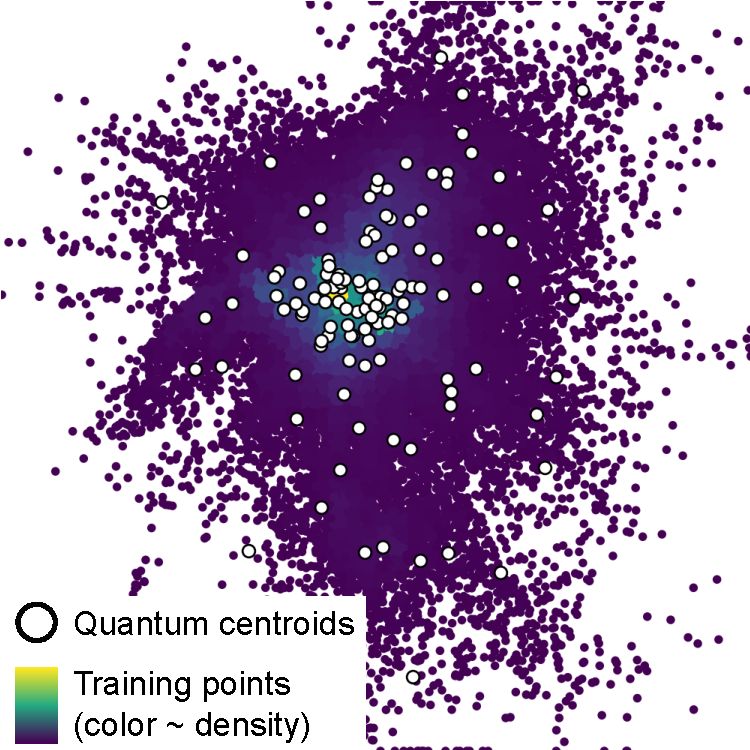
\includegraphics[width=0.45\linewidth]{figures/04_ema/ae_fits/ae_fit_kmeans.pdf}
				}
				\subfloat[BSQ]{
					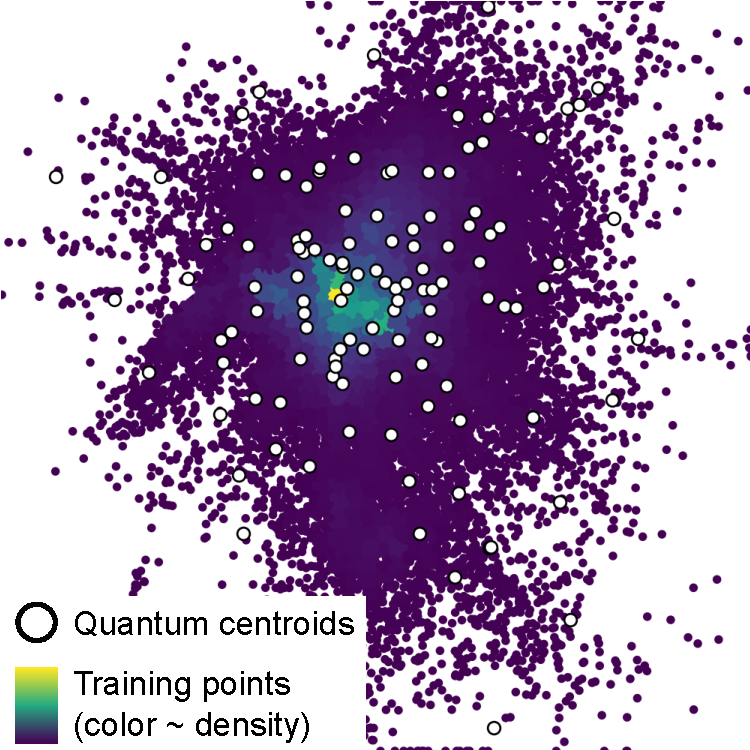
\includegraphics[width=0.45\linewidth]{figures/04_ema/ae_fits/ae_fit_bsq.pdf}
				}
				\caption[Scatterplot of \kmeans{} and BSQ centroids on the EMA dataset]{Scatterplot of \kmeans{} and BSQ quantization on the simulator dataset for $k=120$.}
				\label{fig:ae_fits}
			\end{figure}
			
			The number of fitted quanta (the value $k$) is a user-defined parameter for both algorithms.
			In other clustering tasks, where the goal is to find a logical grouping in the data (logical to a human user), there are theoretically correct $k$ value(s) for each task.
			In these cases, finding the correct $k$ value is crucial to achieving good results, even more so, if the user has a very strong (biased) expectations of how the formed clusters should look.
			Fortunately, this is not the case for the quantization in the \ac{EMA}, because the goal is not to find a logical -- according to a human supervisor -- grouping of the observations.
			In our case, it is sufficient to quantize the input space with a ``fine enough'' resolution so that the mapping stage can work with reasonable precision.
			This criterium does not really pose a hard upper-limit to the number of quanta that can be used.
			The number of possible quanta can be softly limited by:			
			\begin{itemize}
				\item The number of available training points, so that each quantum stays reasonably populated (Sec.~\ref{cha:deep_learning:sec:overfitting}).
				This restriction coincides with the avoidance of overfitting, because underpopulated quanta can easily overfit the data, so that the quantization loses generalization power.
				
				\item The available computational resources, such as memory.
				More quanta used in the computation requires more memory, as well as more computational power, or takes longer to compute.
			\end{itemize} 
			
			Performance for both algorithms was evaluated for $k = 12, 18, 24, ..., 120$.
			For each value of $k$, both algorithms were run $100$ times starting from random initial quantum locations, and the previously explained two evaluation metrics were measured (both metrics for both algorithms).
			The results can be seen in Fig.~\ref{fig:quant_distances}, where shaded regions depict the $\pm1$ standard deviation, solid lines depict the mean.
			
			\begin{figure}[ht]
				\centering
				\subfloat[Average distances]{
					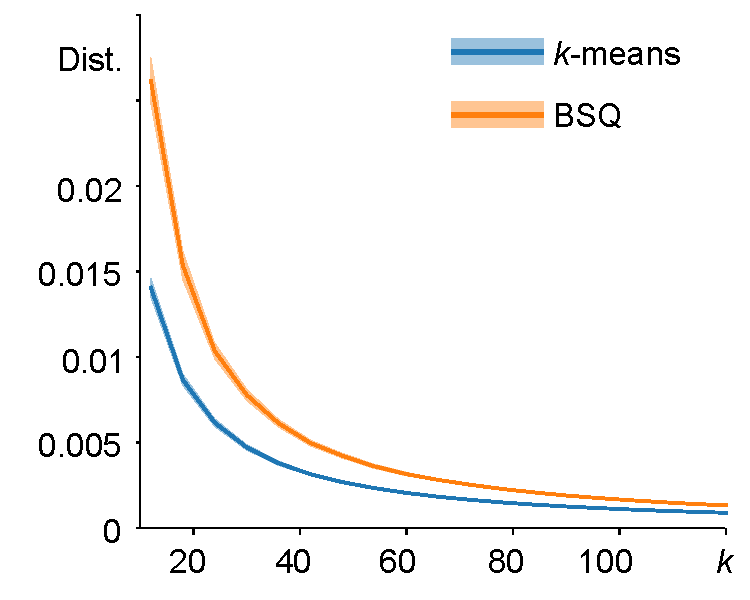
\includegraphics[width=0.45\linewidth]{figures/04_ema/quant_distances/quant_dist_avg_framed.pdf}
				}
				\subfloat[Maximum distances]{
					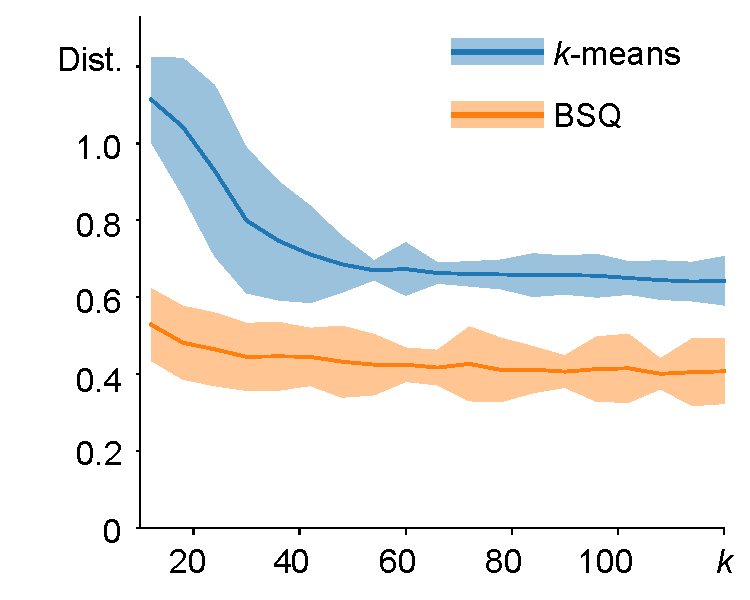
\includegraphics[width=0.45\linewidth]{figures/04_ema/quant_distances/quant_dist_max_framed.pdf}
				}
				\caption[\kmeans{} and BSQ average and maximum distances]{Average and maximum distances measured for multiple $k$ values for \kmeans{} and BSQ.}
				\label{fig:quant_distances}
			\end{figure}
			
			As expected, increasing $k$ achieves a smooth reduction of the average distance for both algorithms, with \ac{BSQ} constantly having $60\%$ larger averages, and both having minimal variance.
			On the other side, \ac{BSQ} achieves $30\%$ smaller average maximum distance at larger values of $k$, and almost $50\%$ smaller average maximum at small values of $k$.
			Generally, the maximum distances for both algorithms show a large variance across all values of $k$.			
		
		\subsection{State Mapping}
			\label{cha:ema:sec:mapping}
		
			Mapping of states, the third component of the \ac{EMA}, enables translation from the objective but abstract internal states to \ac{CF}-specific subjective external states.
			State mapping is essential to convert the output of the quantization, which is the internal state-space model, to well-defined labels, which are understandable by both the human operator and the \acp{CF} in the \ac{CAN} subsequent stages.
			State-mapping is envisioned as a simple labeling task, where a specific ``coloration'' (labeling) of the internal state-space is stored for each dimension/aspect of the output external states.
			Each ``color'' (label) represents a different level of the quantized output dimension.
			
			Ideally, the entirely unsupervised feature reduction and quantization steps produce quanta that are \textit{well-aligned} to any sensible labeling of the dataset if it is to be done by the human operator.
			``Well-aligned'', in this case, implies that each cluster contains mostly observations of a single class/label.
			In practice, this is not necessarily true due to the unsupervised nature of the feature reduction and quantization algorithms, which can produce results that are unfitting to the biased supervised labels produced by the system designer.
			In this study, the class labels are the different settings for the simulated cells.
			As mentioned before, there are only soft upper limits to the number of quanta that can be used in the internal state-space model.
			This is important, because it is assumed that by increasing $k$, the internal states become more and more aligned to any outside labeling, following a sensible curve.
			However, this is not necessarily true, depending generally on the distribution of the different classes, but also specifically on the feature reduction and the fitted states.
			This section tries to answer the question as to whether or not the assumption is correct that increasing $k$ leads to better alignment of the quanta.
		
			State mapping is implemented by assigning the label of the class with the majority population to each internal state.
			If the above assumption is true, by increasing the resolution of the internal state-space (increasing $k$), this alignment should constantly improve until reaching an acceptable level.
			To evaluate the alignment quality, we defined \textbf{state purity} ($P$), an external metric of quantum alignment, measuring the percentage of the majority class (largest population) against the total population within an internal state, i.e.:
			\begin{equation}\label{eq:purity_single}
			P = \sum_{i} \frac{\max_{j} r_{ij}}{\sum_{j} r_{ij}} / k, 
			\end{equation}
			\noindent where $r_{ij}$ is the number of points of class $j$ in state $i$, and $k$ is the number of internal states.
			For $100\%$ purity, each state would contain observations from only one class.
			
			Between the two extremes of $k$, it is not clear how purity changes.
			On one end, using a single state for the whole dataset would yield a purity that is inherent in the class populations in the data.
			On the other end, using a state for every single observation would produce a purity value of a $100\%$.
			However, between these two values, if the change is not gradual, state mapping would be hard to use, as a well-functioning $k$ would be hard to find, or computationally infeasible to use.
			
			\begin{figure}[ht]
				\centering
				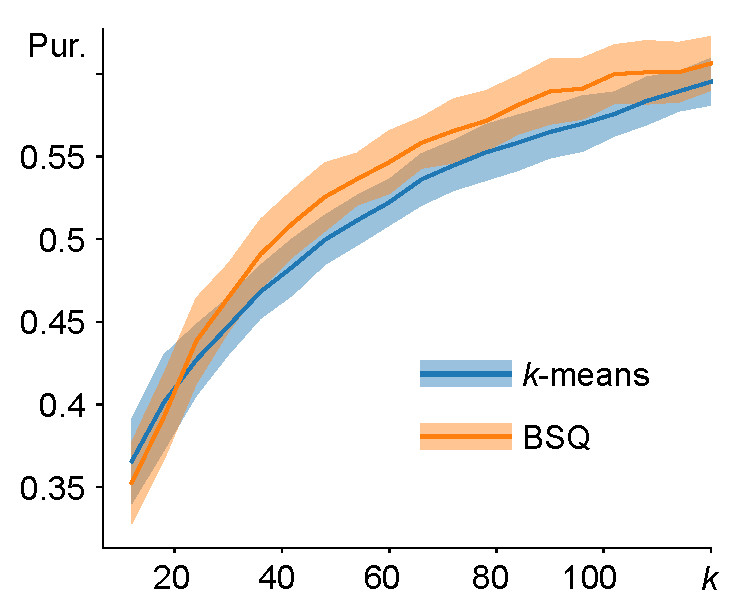
\includegraphics[width=0.5\linewidth]{figures/04_ema/purity_overall/purity_overall_framed.pdf}
				\caption[\kmeans{} and BSQ overall purity]{\kmeans{} and BSQ overall purity for different quantum numbers. }
				\label{fig:purity_overall}
			\end{figure}
		
			Figure~\ref{fig:purity_overall} shows how the overall purity changes depending on $k$, with shaded regions depicting the $\pm1$ standard deviation, solid lines depicting the mean.
			For both algorithms, the average overall purity values steadily increase with increasing $k$, indicating that quantization resolution is well correlated to mapping accuracy.
			Although starting at a lower value, \ac{BSQ} also seems to have a steeper slope in the lower ranges of $k$ compared to \kmeans{}.
			The two averages cross over at $k=24$, after which point \ac{BSQ} has a constant lead up to $k=100$, where this lead starts to diminish.
			The variance seems to keep constant for all the different $k$ values.
			
			Figure~\ref{fig:purity_dist} provides a more insightful look into the distribution of state purity values for both algorithms, for $4$ different $k$ values.
			In the plots, the horizontal axis gives the percentage of purity. We see that for low values of $k$ (blue curve, $k=12$), \kmeans{} has very strong peak densities of purity around $0.25$ and $0.55$, whereas \ac{BSQ} does not have such defined peaks.
			At a high value of $k$ (red curve, $k=120$), both distributions are very similar, however, \kmeans{} seems to have more states which are close to a $100\%$ purity.
			These differences in the distributions reflect the ones that we have already seen for the average state purity previously.
			
			\begin{figure}[ht]
				\centering
				\subfloat[\kmeans{}]{
					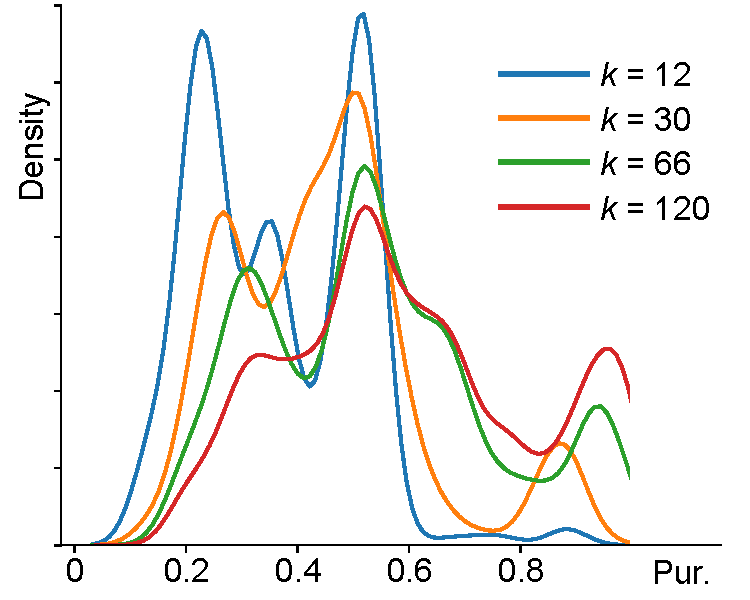
\includegraphics[width=0.47\linewidth]{figures/04_ema/purity_dist/purity_dist_kmeans_framed.pdf}
				}
				\subfloat[BSQ]{
					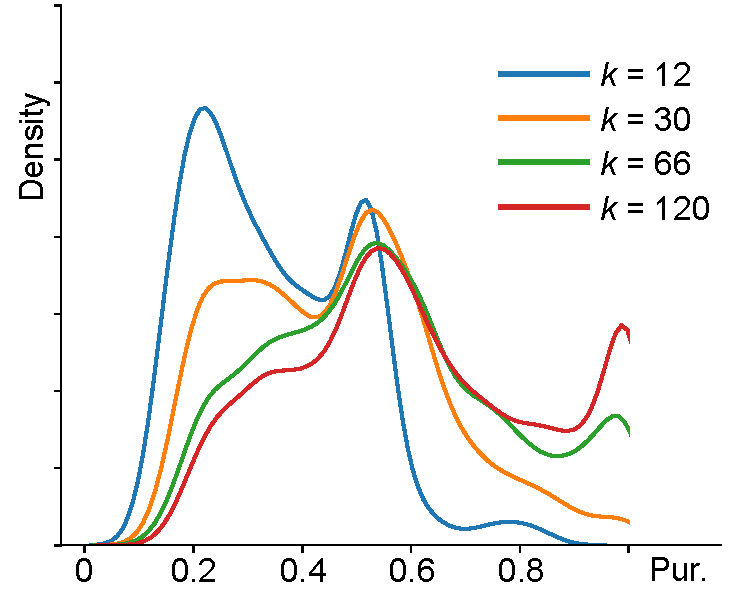
\includegraphics[width=0.47\linewidth]{figures/04_ema/purity_dist/purity_dist_bsq_framed.pdf}
				}
				\caption[State purity distributions in the EMA evaluation]{State purity distribution for $k=12, 30, 66, 120$ quanta.}
				\label{fig:purity_dist}%
			\end{figure}
		
			Figure~\ref{fig:purity_classwise} shows the share average and variance for each class separately for $4$ different values of $k$.
			The horizontal axis gives the class labels, while the vertical axis shows the normalized number of clusters with majority for the specific class, so that $1.0$ equals to having ${1/12}^{th}$ of the clusters as majority.
			Each observation for a specific value of $k$ and class has been plotted on the horizontal axis with a small offset.
			The main takeaway here is that as $k$ increases, the normalized average share for each class tends towards $1.0$, meaning that the majority class labels are more and more evenly distributed between the clusters, with no class having a tendency to not be assigned to any of the clusters (to be ``left out'' of the mapping).
			This is warranted, as originally the class labels occupy a roughly even amount of observations in the dataset.
			
			\begin{figure}[ht]
				\centering
				\subfloat[\kmeans{}]{
					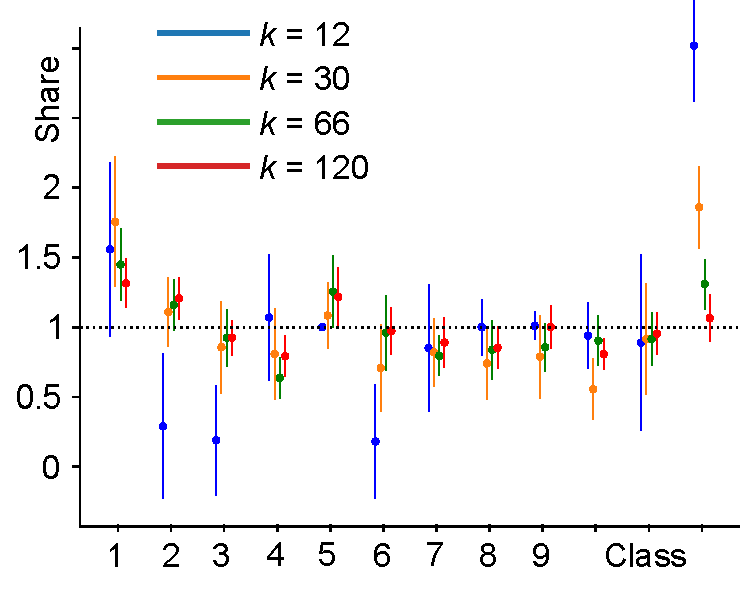
\includegraphics[width=0.47\linewidth]{figures/04_ema/purity_classwise/purity_classwise_kmeans_framed.pdf}
				}
				\subfloat[BSQ]{
					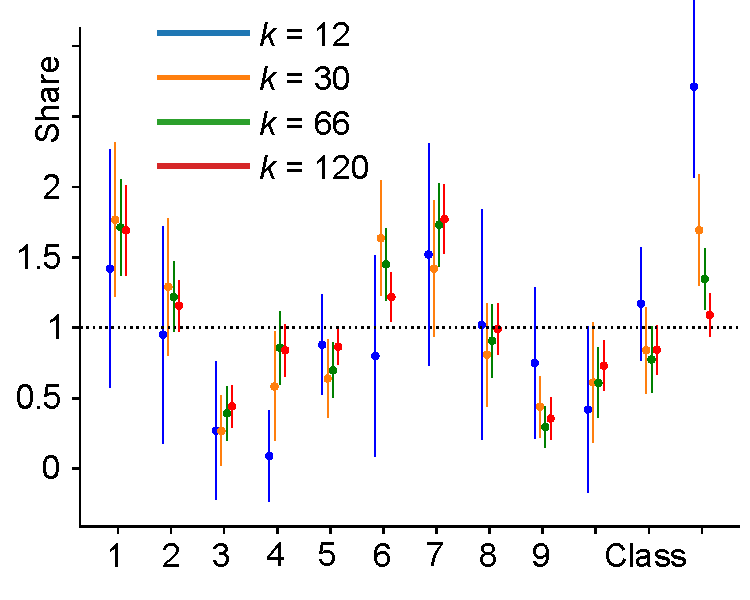
\includegraphics[width=0.47\linewidth]{figures/04_ema/purity_classwise/purity_classwise_bsq_framed.pdf}
				}
				\caption[Cluster shares in the EMA evaluation]{Share of clusters for each class for $k=12, 30, 66, 120$ quanta.}
				\label{fig:purity_classwise}
			\end{figure}
			
			In general, the original assumption of being able to find a good enough mapping accuracy to any sensible labeling of the state-space seems warranted.
			With a larger number of $k$, the simple mapping process of assigning the label of the majority population to the cluster can give an acceptable level of cluster purity.
			When the value of $k$ is constrained, \ac{BSQ} is recommended, otherwise \kmeans{} seems to be the better choice.			
			While this concludes this evaluation, we suspected that even better results could be achieved with regards to cluster purity, if state-of-the-art deep clustering is used for the formulation of the \ac{EISS}, which is the topic of the next section.
			
		\subsection{Conclusion and Critique}
						
			While achieving acceptable results, we were not quite satisfied with the precision of our quantization, thus, we wanted to further refine our method.
			It became clear during the evaluation that network states are often not immediately distinguishable in the data, even through the feature extraction done by the \ac{AE}.
			To rectify this, we thought of using an added constraint from a then newly published paper, which was meant to help the \ac{AE} in learning an encoding in which groups in the data are separated better.
			In the work described in the next section, we revisit the \ac{EMA} engine, and apply a modern deep clustering method to the problem, as well as reevaluating the original \ac{EMA} proposal using deeper, more complex neural nets and a larger simulated dataset.			

	\section{Towards Deep Clustering in EMA}
		\label{cha:ema:sec:ema_acai}
	
		\subsection{Deep Clustering with ACAI}
			
			Deep autoencoders are able to encode observations into a structured view, where neighboring observations share complex correlation structures.
			Unfortunately, often these structured encodings do not lend well to the simple spherical quanta formed by \kmeans{} or \ac{BSQ}.
			It would be possible to use more complex statistical quantization (clustering) methods -- such as \acp{GMM} -- to move away from spherical clusters in order to better fit the encoded observations, as these usually provide better accuracy than \kmeans{}.
			However, these complex quantization methods are often intractable to calculate in many-dimensional spaces or with a large number of classes.
			For example, \kmeans{} in a $10$-dimensional space ($D = 10$) with $10$ quanta ($k = 10$) uses $D*k = 100$ parameters. 
			A \ac{GMM} in the same setting uses $((D*D - D)/2 + 2D) * k = 650$ parameters with full covariance matrices. 
			One can see that the number of parameters can quickly go out of hand by increasing $D$ or $k$. 
			A better approach is to encourage a \kmeans{}-friendly encoding structure in the autoencoder through an additional component or loss. 
			This is the approach that a large portion of the deep clustering neural nets have taken recently.
			
			From a very high level, many deep clustering methods can be seen as a simpler statistical quantization algorithm -- such as \kmeans{} -- and a feature-extraction preprocessing step fused together.
			This fusion is usually helped by additional constraints during training, to make the two methods work well together.
			Depth comes from the complex neural nets that are used for feature extraction.
			The feature-extraction method used in this work is the autoencoder as described in the previous section.
			However, to encourage a \kmeans{}-friendly encoding, an advanced version of the autoencoder setup was evaluated, called \ac{ACAI} from Google Brain \cite{acai}.
			In \ac{ACAI}, a \textit{discriminator} subnet is attached to a deep autoencoder (Fig.~\ref{fig:acai_interpolation}), whose task is to encourage linear transitions in the latent space, which makes the encoding \kmeans{}-friendly.
			To achieve this, the autoencoder decodes artificial observations generated from linear mixtures of pairs of encoded observations with a randomly chosen mixing coefficient $\alpha$, which the discriminator has to guess from the decoded (reconstructed) artificial observation.
			
			\begin{figure}[ht]
				\centering
				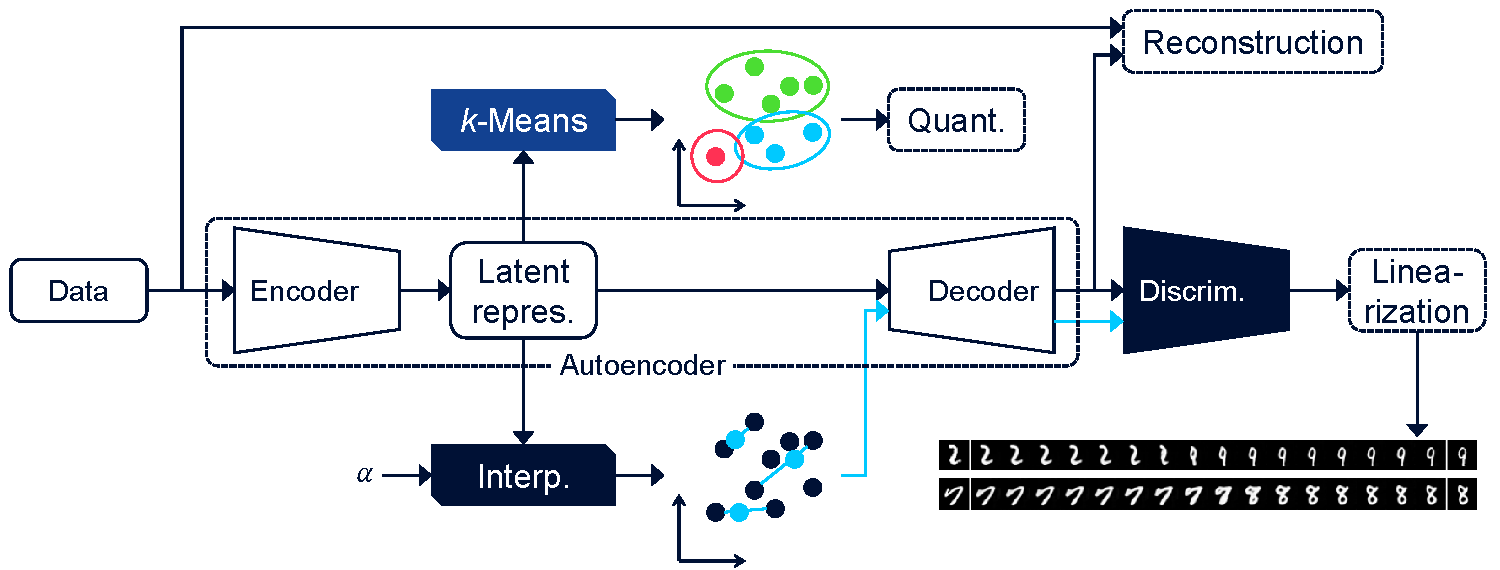
\includegraphics[width=\linewidth]{figures/04_ema/acai_interpolation/acai_interpolation.pdf}
				\caption[Illustration of the ACAI algorithm]{Linearization of the latent space in ACAI through the GAN training structure.}
				\label{fig:acai_interpolation}
			\end{figure}
			
			The autoencoder and the discriminator are adversaries, with the autoencoder working against the discriminator by trying to make the mixing coefficient hard to guess, in addition to trying to minimize the traditional autoencoder reconstruction loss. 
			Together, the autoencoder and the discriminator form a \ac{GAN} training structure (Sec.~\ref{cha:deep_learning:sec:gan}).
			Intuitively, if the encoding space does not contain linear transitions, the artificial observations are easy to distinguish from actual observations, which makes it easy for the discriminator to guess the mixing coefficient with simple rules and high precision. 
			To counteract this, the autoencoder can try to make the artificial observations ``look like'' actual observations. 
			Because artificial observations are generated with a random mixing coefficient, this means that anywhere in the encoded manifold, points have to decode into believable observations. 
			Theoretically, both the reconstruction and mixing losses can be minimized by the autoencoder, as these are not conflicting goals.
			However, the extent largely depends on the capabilities of the encoder, decoder and discriminator subnets.
			In the case of neural nets, modeling capability is mostly set by net topology, and in our case, the subnets are deep, containing many layers, and thus are very capable. 
			As advised by the original paper, the discriminator has the same layer topology as the encoder, the only difference being an extra averaging layer at the end to arrive at a single value as the output $\alpha$, while the decoder is roughly a mirror equivalent of the encoder.	
			
			After \ac{ACAI} is trained, all but the encoder subnet can be discarded, and the encoder used to translate the observable network state into a clustering-friendly space. 
			Although any clustering method could be used, the most obvious choice (and the one the \ac{ACAI} paper originally uses) is the \kmeans{} algorithm. 
			One major difference between the original intended use for \kmeans{} in \ac{ACAI} and our use case is that what we are doing is not strictly clustering. 
			In the \ac{ACAI} paper, the number of quanta (the parameter $k$) is set to be equal to the number of suspected groups in the data. 
			On one hand, this a-priori requirement is always questionable, as in realistic settings usually it is unknown how many groups are present in the dataset, and clustering is used in an exploratory fashion. 
			On the other hand, the envisioned \ac{EISS} representation does not require that a network state is only contained in a single quantum. 
			Once again, this allows us to set $k$ to an arbitrary, large enough number, with only soft constraints; $k$ should be larger or equal than the number of network states present in the data, but small enough so that all quanta (internal states) are reasonably populated from the training dataset.
				
	
		\subsection{Differences in Simulation Environment, Data and Net Topology}
		
			This work revisits the same concepts that have been discussed in Sec.~\ref{cha:ema:sec:ema_bsq}, and will be referred to as ``previous'' evaluation.
			The overall method of evaluation is the same: the task of the \ac{EMA} engine is to extract descriptive features, and form quanta for the \ac{EISS} which also align to existing groups in the measurements.
			The biggest differences between the previous evaluation and the one shown here are the inclusion of the \ac{ACAI} algorithm, and the exclusion of \ac{BSQ}.
			\ac{BSQ} was chosen not to be evaluated again, because it seemed to only provide marginal improvements over \kmeans{} in the \ac{EMA} context.
			The exclusion of \ac{BSQ} sped up the evaluation process, as well as spared us from having to explain how it functions in the already limited space these results were published in.
			
			Similarly to our previous evaluation, a dataset from a controlled network and environment was needed, one that contained known classes (groups) that are discoverable by the environment modeling system.
			To generate such a dataset, the same network-level simulator was used in a similar scenario as described before.
			The classes for the evaluation were formed by cells sharing similar parameter setting combinations. 
			Although this is not realistic as cell parameter settings would be known to the operator in a real network deployment, it helps us evaluate the \ac{EMA} concept; the parameters are meant to mimic different user behaviors and environmental conditions that might affect the network and are outside of the operators control.
			The simulation scenario contained a number of $3$-sector \ac{LTE} macro ($2$ GHz), omnidiricetional \ac{LTE} micro ($2.6$ GHz), and WiFi ($2.4$ GHz) cells.
			Three parameters were iterated to form $12$ setting groups as shown in Tab.~\ref{tab:cell_params_2}, these were the \ac{RSRP} offset, \ac{TTT} and \ac{TXP}.
			Compared to the previous scenario, notable differences here were changes made to \ac{RSRP} and \ac{TTT} values, which made the setting classes a little more distinguishable.
			The WiFi network using the \ac{TTT} parameter was not really realistic, which was changed in this evaluation to the \ac{RSRP} offset.
			
			The output of the simulator was made up of $17$ transceiver-level measurements (\acp{KPI}) for each cell.
			The number of \acp{KPI} is lower than in our previous evaluation, as we have forgone the feature-engineering of aggregated \acp{KPI} relating to cell-neighbor behavior.
			Here, only measurements about a single cell were contained in an observation.
			The reported \acp{KPI} pertain to radio condition, cell load and handover behavior, with some \acp{KPI} representing the number of times a specific action occurred (such as a late handover), while others average a measured value (such as \ac{RSRP}) over the reported time period.
			The frame length of the simulation was again $0.1$ ms, but the \acp{KPI} were aggregated to a much larger granularity period of $5$ simulated minutes compared to the previous $15$ second periods.
			To counteract this larger aggregation window, the simulation ran for a much longer time than in the previous evaluation, resulting in $72$ thousand records collected over roughly one and a half weeks of simulated network operation.
			
			\begin{table}[t]
				\renewcommand*{\arraystretch}{1.2}
				\centering
				\begin{tabular} {l|c c c c c c c c}
					& \multicolumn{8}{c}{LTE Macro} \\ 
					\hline
					Setting 			& M$_{1}$	& M$_{2}$	& M$_{3}$	&	M$_{4}$	& M$_{5}$	& M$_{6}$	& M$_{7}$	& M$_{8}$	\\
					\hline 
					RSRP offset [dB] 	& 1.0		& 3.0		& 3.0		& 1.0		& 1.0		& 3.0		& 3.0		& 1.0		\\
					TTT [s]				& 0.512		& 0.512		& 0.512		& 0.512		& 1.02		& 1.02		& 1.02		& 1.02		\\
					TXP [dBm]			& 46		& 46		& 40		& 40		& 46		& 46		& 40		& 40		\\
					\hline						
					& \multicolumn{2}{c|}{LTE micro} 			& \multicolumn{2}{c}{WiFi} 			& & & & \\
					\cline{1-5}
					Setting 			& m$_1$	& \multicolumn{1}{c|}{m$_2$}		& W$_1$	& \multicolumn{1}{c}{W$_2$}	& & & & \\
					\cline{1-5} 
					RSRP offset [dB] 	& 1.0	& \multicolumn{1}{c|}{3.0}			& 1.0	& \multicolumn{1}{c}{1.0}	& & & & \\
					TTT [s]				& 0.512	& \multicolumn{1}{c|}{1.02}			& -		& \multicolumn{1}{c}{-}		& & & & \\
					TXP [dBm]			& 20	& \multicolumn{1}{c|}{20}			& 20	& \multicolumn{1}{c}{24}	& & & & \\
				\end{tabular}
				\caption[Cell parameters in the renewed EMA simulation]{Cell parameter combinations in the renewed simulations}
				\label{tab:cell_params_2}
			\end{table}
			
			The modeling capability of the \ac{EMA} engine largely depends on the complexity of the encoder, decoder and discriminator subnets.
			In the case of neural nets, modeling capability is mostly set by net topology, and in our case, the subnets are deep, containing many layers, and thus are very capable. 
			As advised by the original \ac{ACAI} paper, the discriminator used the same layer topology as the encoder, the only difference being an extra averaging layer at the end to arrive at a single value as the output $\alpha$, while the decoder is roughly a mirror equivalent of the encoder.
			The topologies of the subnets can be seen in Fig.~\ref{fig:acai_topology}.
			These neural nets were much deeper compared to their counterparts in our previous experiment, which can also explain some of the improvement seen in the state purity achieved in the evaluation.
			The topology is also different in its overall shape: where in the previous evaluation, the autoencoders were constricting information flow by continuously reducing the number of neurons towards the middle of the \ac{AE}, here the number of neurons actually increases towards the middle, all up until the very middle layers, which abruptly reduce the number of dimensions to a very low value.
			This shape had a very good effect on the reconstruction accuracy, and allowed the \ac{AE} to more consistently map similar observations close together in the latent (encoding) space.
			First used here, this general shape for an \ac{AE} is reused in many of our experiments, as we will see in later chapters.
			
			\begin{figure}[ht]
				\centering
				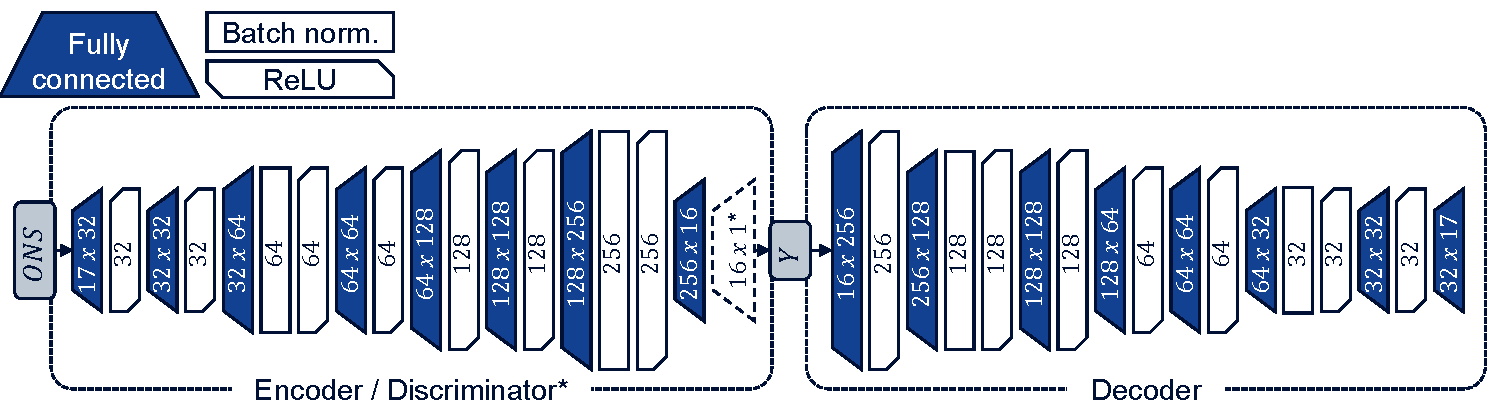
\includegraphics[width=\linewidth]{figures/04_ema/acai_topology/acai_topology.pdf}
				\caption[AE topologies in the renewed evaluation]{Neural net topologies of the subnets used.}
				\label{fig:acai_topology}
			\end{figure}
			
		\subsection{Evaluation}
			
			In this evaluation, \kmeans{} quantizations are fit: 1) on the raw data without feature extraction, 2) on the features extracted using a traditional autoencoder (with the same topology as shown in Fig.~\ref{fig:acai_topology}), and 3) on the features extracted using \ac{ACAI}.
			As \kmeans{} is sensitive to initialization and is initialized randomly, we repeat the quantization for every $k$ value $30$ times.
			This is also represented in the results in Fig.~\ref{fig:pur_dist}, where instead of singular purity values, distributions are shown.

			\begin{figure}
				\centering
				\subfloat[Purity overview.]{
					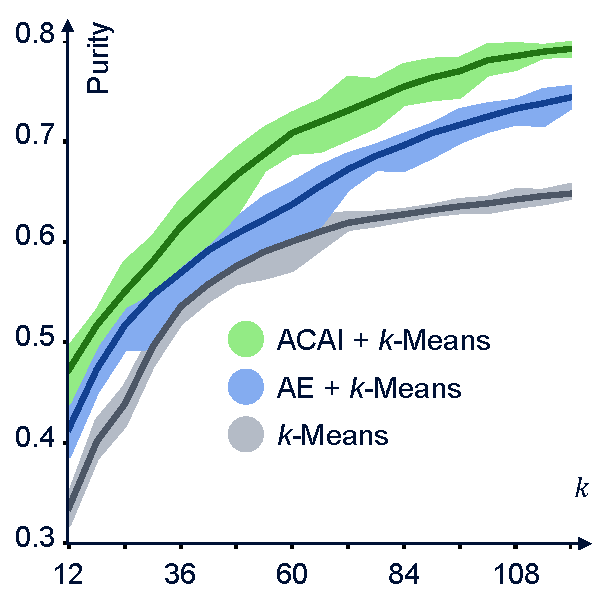
\includegraphics[width=0.4\linewidth]{figures/04_ema/pur_dist/pur_overview.pdf}
					\label{fig:pur_overview}
				} \\
				\subfloat[Distr. at $k = 12$.]{
					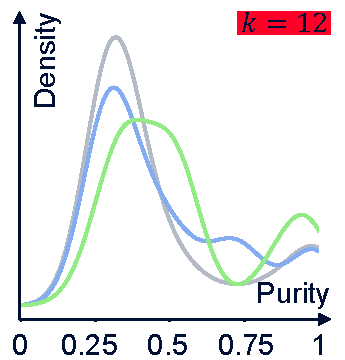
\includegraphics[width=0.23\linewidth]{figures/04_ema/pur_dist/pur_dist_k012.pdf}
					\label{fig:pur_dist_k012}
				}				
				\subfloat[Distr. at $k = 36$.]{
					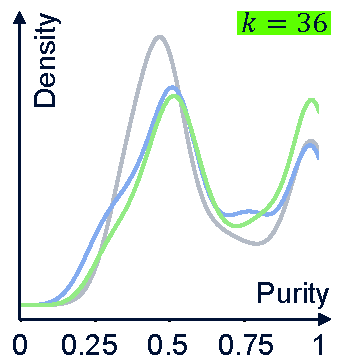
\includegraphics[width=0.23\linewidth]{figures/04_ema/pur_dist/pur_dist_k036.pdf}
					\label{fig:pur_dist_k036}
				}
				\subfloat[Distr. at $k = 72$.]{
					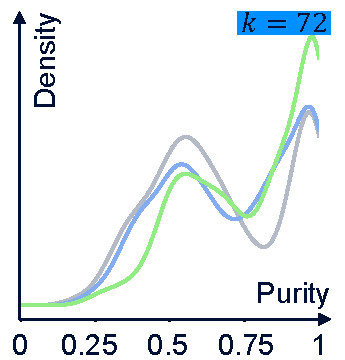
\includegraphics[width=0.23\linewidth]{figures/04_ema/pur_dist/pur_dist_k072.pdf}
					\label{fig:pur_dist_k072}
				}
				\subfloat[Distr. at $k = 120$.]{
					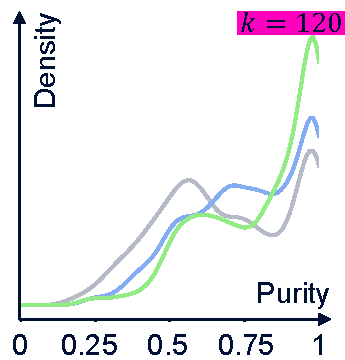
\includegraphics[width=0.23\linewidth]{figures/04_ema/pur_dist/pur_dist_k120.pdf}
					\label{fig:pur_dist_k120}
				}
				\caption[State purities in the renewed EMA evaluation]{State purity at different $k$ values.}
				\label{fig:pur_dist}
			\end{figure}
			
			Figure~\ref{fig:pur_dist} shows how state purity changes by increasing $k$.
			Subfigure~\ref{fig:pur_overview}, highlights the purity values across all $k$ values for the $3$ clustering methods. 
			Solid lines depict the average, while bands run from the minimum to the maximum values.
			Although none of the methods produce particularly good purity at lower $k$ values, at high values of $k$ \ac{ACAI} reaches almost $0.8$ purity, with the traditional autoencoder trailing behind at around $0.73$. 
			This gain might not seem much, but in terms of erroneously clustered points, the difference between an autoencoder and the \ac{ACAI} is a $24\%$ reduction. 
			Native \kmeans{} without feature extraction levels out at around $0.6$ purity, and starts to not scale well above $k=48$.	
			Subfigures~\ref{fig:pur_dist_k012} - \ref{fig:pur_dist_k120} provide a better look into the distribution of purity at $k$ values $12$, $36$, $72$ and $120$ respectively.
			It is interesting to note that \ac{ACAI} seems to have more high-purity clusters all through the $k$ range than the other methods.
			
			\begin{figure}
				\centering
				\subfloat[\kmeans{}]{
					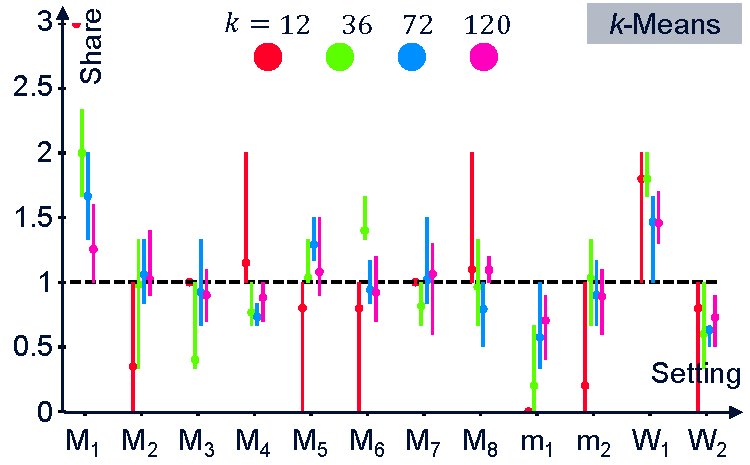
\includegraphics[width=0.48\linewidth]{figures/04_ema/class_shares/class_shares.pdf}
					\label{fig:class_shares}
				} \\
				\subfloat[AE + \kmeans{}]{
					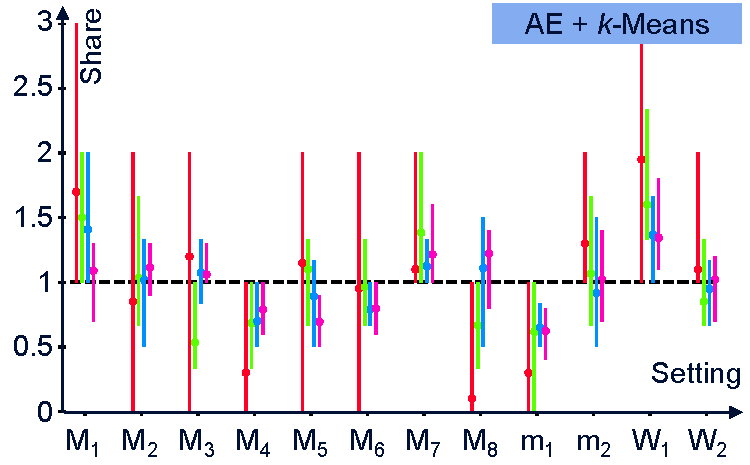
\includegraphics[width=0.48\linewidth]{figures/04_ema/class_shares/class_shares_ae.pdf}
					\label{fig:class_shares_ae}
				}
				\subfloat[ACAI + \kmeans{}]{
					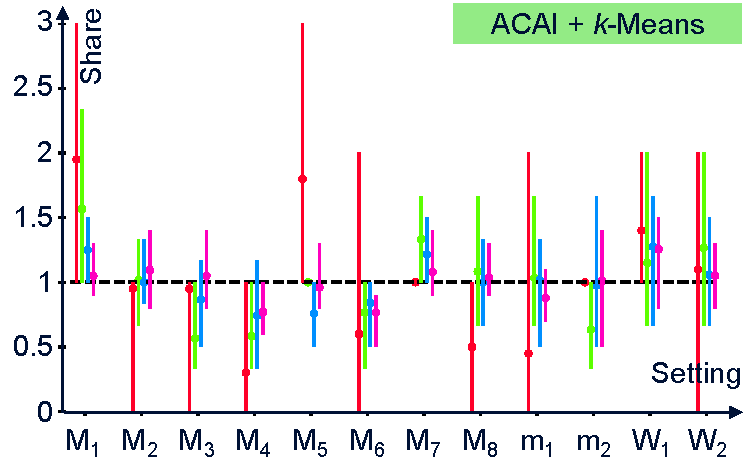
\includegraphics[width=0.48\linewidth]{figures/04_ema/class_shares/class_shares_acai.pdf}
					\label{fig:class_shares_acai}
				}	
				\caption[Class majority shares in the renewed EMA evaluation]{Class majority shares for the different feature extraction methods.}
				\label{fig:shares}
			\end{figure}
			
			Figure~\ref{fig:shares} shows, for each class, the normalized number of clusters that have that class as majority.
			Here, $1.0$ share means the class occupies $1/12$ of the clusters as majority.
			Dots represent the average, lines run from the minimum to the maximum values, and colors correspond to the different $k$ values.
			Generally, all class-shares seem to converge towards $1.0$ as $k$ increases.
			This is important, as no class is ``dissolved'' among the others, and so each will get its own fair share of clusters with a sufficiently large $k$.
			This is most true for \ac{ACAI}, which seems to best converge towards $1.0$ share.
			
			All-in-all, deep clustering using a combination of the \ac{ACAI} and the \kmeans{} algorithms is able to distinguish underlying (hidden) groups in the dataset.
			The quantization for the \ac{EISS} produced results with high accuracy at the $k$ value of $120$, which is still well within computational feasibility.
			While the differences in simulation, data and net topologies makes these results incomparable to our previous results, it is evident that the concept of environment modeling seems feasible, and the \ac{ACAI} algorithm is a strong candidate for the modeling of network and environment states.
		
		\subsection{Conclusion}

			This chapter discussed a candidate design (called \ac{EMA}) for modeling of objective network states (\ac{EIS}), and the abstraction of subjective discrete states (\ac{DAS}) from the objective network states.
			The network states mapped in the \ac{EISS} can be used as a basis for communication between \acp{CF} and other components in the \ac{CAN}.
			The fine quantization in the \ac{EISS} allows for a simple mapping procedure where individual actions, or \ac{CF}-specific states can be assigned to whole \ac{EIS} states, simplifying a lot of potential modeling complexity in the \acp{CF}, and hopefully keeping them lightweight.
			However, it became clear that the quantization cannot be simply done without regard to present contextual (hidden/latent) groups in the data, as these can invalidate the abstraction/mapping procedure.
			If the \ac{EIS} states incorporate multiple contextual groups into a single state, logically, the mapping will be incapable to assign accurate actions or meaning to these states.
			
			In order to see how big of a problem this is, and how well the alignment of \ac{EIS} states to contextual groups improve by increasing the number of \ac{EIS} states, we have evaluated the \ac{EMA} concept on simulated datasets.
			Our evaluation showed that -- using various feature extraction methods -- the quantization that forms the \ac{EIS} states can be aligned to a very high accuracy to contextual states.
			The best performing method in this regards was the \ac{ACAI} algorithm, which tries to integrate the feature extraction into the quantization process by influencing the way the extracted features are formed.
			So far, the feature extraction step was seen as a separate preprocessing step which helps the quantization to combat noise, as well as the curse of dimensionality.
			However, it is clear that the feature extraction steps plays a crucial role in the correct understanding/modeling of the network behavior, thus should handled as a single processing step, together with the quantization.
			In fact, the feature extraction and quantization algorithms should be tailored to work with each other, paving the way towards deep clustering, which is the focus of the next part of this thesis.
		